%%%%%%%%%%%%%%%%%%%%%%%%%%%%%%%%%%%%%%%%%%%%%%%%%%%%%%%%%%%%%%%%%%%%%%%%
%                                                                      %
% LaTeX, FIIW thesis template                                          %
% 28/11/2014 v1.2                                                      %
%                                                                      %
%%%%%%%%%%%%%%%%%%%%%%%%%%%%%%%%%%%%%%%%%%%%%%%%%%%%%%%%%%%%%%%%%%%%%%%%
\documentclass[11pt,a4paper]{report}
% Indien je je thesis recto-verso wil afdrukken gebruik je onderstaande opties i.p.v. bovenstaande
%\documentclass[11pt,a4paper,twoside,openright]{report}

\usepackage[a4paper,left=3.5cm, right=2.5cm, top=3.5cm, bottom=3.5cm]{geometry}
\usepackage[english]{babel}
\usepackage{graphicx}
%\usepackage[latin1]{inputenc}           % om niet ascii karakters rechtstreeks te kunnen inputten
\usepackage[utf8]{inputenc}            % commentarieer deze regel uit als je utf8 encoded files gebruikt in plaats van latin1
\usepackage[numbers]{natbib}
\usepackage{listings}             		% voor het weergeven van broncode
\usepackage{verbatim}					% weergeven van code, commando's, ...
\usepackage[hidelinks]{hyperref}		% maak PDF van de thesis navigeerbaar without boxes
%\usepackage{hyperref}					% maak PDF van de thesis navigeerbaar
\usepackage{url}						% URL's invoegen in tekst met behulp van \url{http://}
\usepackage[small,bf,hang]{caption}     % om de captions wat te verbeteren
\usepackage[final]{pdfpages}            % gebruikt voor het invoegen van het artikel in pdf-formaat
\usepackage{pslatex}					% andere lettertype's dan de standaard types
\usepackage{lipsum}
\usepackage{sectsty}					% aanpassen van de fonts van sections en chapters
%\usepackage[nottoc,numbib]{tocbibind}	% Bibliography mee in de ToC
\usepackage{tikz}
\usepackage{xcolor}
\usepackage{standalone}
\usepackage{enumitem}
\usepackage{multirow}
\setlist{nosep}
%\usetikzlibrary{external}

\allsectionsfont{\sffamily}
\chapterfont{\raggedleft\sffamily}

\usepackage{float}                      % De optie H voor de plaatsing van figuren op de plaats waar je ze invoegt. bvb. \begin{figure}[H]
%\usepackage{longtable}					% tabellen die over meerdere pagina's gespreid worden
%\usepackage[times]{quotchap}           % indien je fancy hoofdstuktitels wil
%\usepackage[none]{hyphenat}
%\usepackage{latexsym}
\usepackage{amsmath}
\usepackage{amssymb}

% MFA: zet zoekpad voor figure
\graphicspath{{fig/}}

\usepackage{fiiw}

%door onderstaande regels in commentaar te zetten, of op false, kan je pagina's weglaten
%bijvoorbeeld het weglaten van een voorwoord, lijst met symbolen, ...
%%%%%%%%%%%%%%%%%%%%%%%%%%%%%%%%%%%%%%%%%%%%%%%%%%%%%%%%%%%%%%%%%%%%%%%%%%%%%%%%%%%%%%%%
%voorwoord toevoegen?
%\acknowledgementspagetrue
\acknowledgements{voorwoord}			%.tex file met daarin het voorwoord

%samenvatting toevoegen
\summarypagetrue
\summary{samenvatting}					%.tex met daarin de samenvatting

%abstract toevoegen?
\abstractpagetrue
\abstracts{abstract}					%.tex file met daarin het abstract
%lijst van figuren toevoegen?
%\listoffigurespagetrue
%lijst van tabellen toevoegen?
%\listoftablespagetrue
%lijst van symbolen toevoegen?
%\listofsymbolspagetrue
\listofsymbols{symbolen}				%.tex file met daarin de lijst van symbolen



%informatie over het eindwerk, de promotor, ...
%%%%%%%%%%%%%%%%%%%%%%%%%%%%%%%%%%%%%%%%%%%%%%%
\opleiding{E-ICT}
\afdeling{Software Engineer}

\campus{denayereng} %denayer,denayereng,geel,geeleng,gent,ghenteng,groept,groupteng,brugge,brugeseng

\title{Counting shells}
\subtitle{Are current neural networks performant enough to count various types of shells in an uncontrolled environment}
% \author{naam student}
\forenameA{ }
\surnameA{ }

% l
\forenameB{Tijs}
\surnameB{Van Kampen}

\academicyear{2022 - 2023}

\promotorA[Promotor]{Prof. dr. Toon Goedemé}

\begin{document}
%\selectlanguage{dutch} %due to incompatible syntax with the English style library and the extended features of the dutch library, I'll be modifying the dutch library to be English
\selectlanguage{english} % For the English version
\preface

%%%%%%%%%%%%%%%%%%%%%%%%%%%%%%%%%%%%%%%%%%%%%%%%%%%%%%%%%%%%%%%%%%% 
%                                                                 %
%                            CHAPTER                              %
%                                                                 %
%%%%%%%%%%%%%%%%%%%%%%%%%%%%%%%%%%%%%%%%%%%%%%%%%%%%%%%%%%%%%%%%%%% 

\chapter{Introduction}

Every year, one day per year, nearly a thousand volunteers travel to the Belgian coast to collect and categorize the shells that wash up on the beach. This data is collected by the flemish institute for the sea (VLIZ) to study populations of marine molluscs and the impact of their environment (climate change, fishing, etc) on the population. The volunteers participating in this study are mostly enthusiasts, but also scientists and families with children. To ensure a good quality of the data, most volunteers participate in a workshop. The counting of the shells is done by walking along the beach and noting every shell that is found individually. This is a very time consuming process, and the volunteers are often not very experienced in counting, resulting in mistakes with all but the most common shells. When a volunteer finds a shell that they are not familiar with, they can contact a helpdesk to help them. The flowchart of the current process can be found in figure \ref{fig:1_current_scenario}. Marked blue are the volunteer's actions, marked red are the parts that involve experts.

\begin{figure}[h]
	\centering
	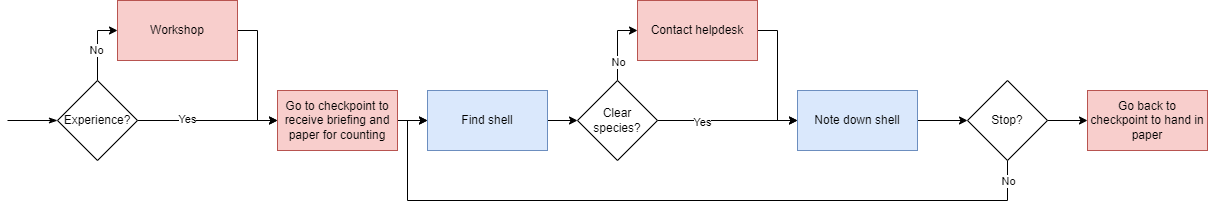
\includegraphics[width=0.8\textwidth]{1_current_scenario}
	\caption{\label{fig:1_current_scenario} The current process of collecting data.}

\end{figure}

The fact that the project relies on volunteers to do most of the legwork, combined with the fact that experts have to man the checkpoints and the helpdesk, makes the project unscalable beyond having a single dedicated day per year. With over 5 million people
%https://www.kustportaal.be/nl/toerisme-en-recreatie#:~:text=De%20Belgische%20kust%20is%20de,in%20totaal%2027.723.420%20overnachtingen.
visiting the Belgian coast every year, there is a lot of potential to collect more data if the process of collecting the data could be simplified to be accessible to anyone visiting the beach at any time.

In this thesis, we will attempt to simplify the process of collecting data so that it can be done by anyone, anywhere, at any time. We will do this by training a counting network to recognize shells in an image and count them automatically. This is already done on a smaller scale by VLIZ with obsidentify. Obsidentify is a mobile app and website where users can submit pictures of a single shell and get a result of what kind of shell it is. This is a useful tool, but taking a close up picture of every single shell is a very time consuming process. We will have to work with a limited dataset to train the neural network as no dataset exist with large quantities of annotated pictures of beaches. After successful completion of this thesis, the new ideal scenario for collecting data can be found in figure \ref{fig:1_ideal_scenario}. Compared to the current process, found in figure \ref{fig:1_current_scenario}, this new process nearly eliminates the experts involvement and thus makes the process scalable.

\begin{figure}[h]
	\centering
	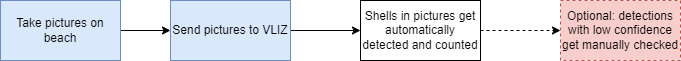
\includegraphics[width=0.8\textwidth]{1_ideal_scenario}
	\caption{The new process of collecting data.}
	\label{fig:1_ideal_scenario}
\end{figure}

We will be studying if current counting networks are performant enough to recognize shells in beach image. We will build up to this by first training a network to count objects from a more established dataset in order to have a baseline to compare our model to. Afterwards we will then train that network with a small dataset to count shells and study its performance.

In the remainder of this thesis we will first discuss the state of the art in the field of object detection and counting, with a focus on few-shot learning. We will then discuss the datasets and the network architecture we will be using. In the second semester we will implement the network and train it on the datasets. We will then discuss the results and the limitations of our model. Finally we will discuss the future work that can be done to improve the model.
%%%%%%%%%%%%%%%%%%%%%%%%%%%%%%%%%%%%%%%%%%%%%%%%%%%%%%%%%%%%%%%%%%% 
%                                                                 %
%                            CHAPTER                              %
%                                                                 %
%%%%%%%%%%%%%%%%%%%%%%%%%%%%%%%%%%%%%%%%%%%%%%%%%%%%%%%%%%%%%%%%%%% 

\chapter{Litature Review}

\section{State of the art/related work}
De masterproeftekst vormt de kern van de scriptie. De tekst wordt logisch opgedeeld in een aantal hoofdstukken. Het eerste hoofdstuk is altijd een inleiding, het tweede en eventueel derde de literatuurstudie of een \textit{state of the art}, gevolgd door een hoofdstuk dat de methodologie beschrijft. De volgende hoofdstukken bevatten de elementen van het eigen onderzoek. Het laatste hoofdstuk bevat de algemene besluiten van de masterproef. Elk hoofdstuk vormt een afgerond geheel (m.a.w. met inleiding en conclusie!).

\section{Verdere onderverdeling binnen een hoofdstuk}
De tekst wordt onderverdeeld in logische paragrafen met een aangepaste nummering. De nummering van de onderliggende delen van een hoofdstuk bevat begint steeds met het hoofstuknummer en gaat maximum tot drie subniveaus. 
Volgende onderverdeling wordt gebruikt:

\section{Dit is een voorbeeld van een sectie}

\subsection{Dit is een voorbeeld van een subsectie}

\subsubsection{Dit is een voorbeeld van een subsubsectie}

\paragraph{Dit is een voorbeeld van een paragraaf}

%%%%%%%%%%%%%%%%%%%%%%%%%%%%%%%%%%%%%%%%%%%%%%%%%%%%%%%%%%%%%%%%%%% 
%                                                                 %
%                            CHAPTER                              %
%                                                                 %
%%%%%%%%%%%%%%%%%%%%%%%%%%%%%%%%%%%%%%%%%%%%%%%%%%%%%%%%%%%%%%%%%%% 
 
\chapter{Implementation}
In this chapter, we will discuss the implementation of the network. We will first discuss the dataset and network architecture we will be using. We will then go into detail about the implementation of the network and the training process. 

\section{Dataset}
In this section, we will go over the datasets used in this paper, with a focus on the shell dataset we are introducing ourselves. With this information, we can better choose candidate models for our task.

\subsection{COCO}

Microsoft's Common Objects in Context (COCO) dataset is a large-scale object detection and segmentation dataset. It contains 330K images with 1.5M instance annotations of 80 different classes. It is split into a training set of 118K images, a validation set of 5K images and a test set of 40K images(the other images are unlabeled). \citet{COCO}

\subsection{Shells}

The shell dataset is a new dataset we are introducing ourselves. As of this writing, it contains 300 images of shells, with 0 annotations. The images shot taken with a cellphone camera on the Belgian coast. Depending on the chosen model, either all images will be annotated or the dataset can be expanded with more images.

This section will be expanded on in the future when annotations are made and the dataset is possibly expanded.

%%%%%%%%%%%%%%%%%%%%%%%%%%%%%%%%%%%%%%%%%%%%%%%%%%%%%%%%%%%%%%%%%%%% 
%                                                                 %
%                            CHAPTER                              %
%                                                                 %
%%%%%%%%%%%%%%%%%%%%%%%%%%%%%%%%%%%%%%%%%%%%%%%%%%%%%%%%%%%%%%%%%%% 
\chapter{Richtlijnen voor formules}

Er zijn twee manieren om formules in LaTeX in te voeren:

\begin{itemize}
	\item Inline: $a^2+b^2 = c^2$ (\verb|$a^2+b^2 = c^2$|)
	\item In een equation omgeving 	(\verb|\begin{equation}	a^2+b^2 = c^2	\end{equation}|):
	\begin{equation}
		a^2+b^2 = c^2
	\end{equation}

\end{itemize}

Griekse letters geef je in d.m.b. het backslash commando. Bijvoorbeeld de letter sigma $\sigma$ verkrijg je door \verb|$\sigma$| inline in te geven. Dit is analoog voor griekse letters in de equation omgeving. Een beknopte lijst van symbolen vind je op de Wikibooks pagina voor LaTeX (\href{https://nl.wikibooks.org/wiki/LaTeX/Wiskundige_formules}{link}). Alle andere nuttige informatie omtrent het gebruik van LaTeX voor formules vind je hier ook terug.
\cleardoublepage
%%%%%%%%%%%%%%%%%%%%%%%%%%%%%%%%%%%%%%%%%%%%%%%%%%%%%%%%%%%%%%%%%%%% 
%                                                                 %
%                            CHAPTER                              %
%                                                                 %
%%%%%%%%%%%%%%%%%%%%%%%%%%%%%%%%%%%%%%%%%%%%%%%%%%%%%%%%%%%%%%%%%%% 
\chapter{Richtlijnen voor referenties}

\section{Inleiding}
De referentielijst bevat de volledige lijst van literatuur en bronnen waarnaar in de tekst wordt verwezen. Door systematisch de referentielijst aan te vullen bij het schrijven van het literatuuroverzicht gaat er achteraf geen tijd verloren aan het opnieuw opzoeken van referenties.

\section{Referentiestijl}

Voor het verwijzen naar informatiebronnen wordt gebruik gemaakt van het numerisch systeem  of van het auteur-jaar systeem. Dit kies je door volgend commando in het latex bronbestand aan te passen:

\begin{itemize}
	\item numerisch (IEEE) : \verb|\bibliographystyle{ieee}|
	\item alfabetisch (APA) : \verb|\bibliographystyle{apalike}|
\end{itemize}

Plaats je bronnen in een \textit{bibtex} bestand (evt. via software zoals bv. Jabref Endnote of Mendeley), waarnaar je verwijst vanuit je thesis text a.d.h.v. het commando \verb|\cite|. Enkele links naar nuttige software in deze context:

\begin{itemize}
	\item \href{http://www.jabref.org/}{JabRef (Open Source)}
	\item \href{http://www.mendeley.com}{Mendeley (Freeware)}
	\item \href{http://www.endnote.com}{EndNote (Paid license)}
\end{itemize}

Indien je zelf een .bibtex bestand wil aanleggen dien je volgende syntax te volgen voor een tijdschriftartikel:
\clearpage
\verb|@article{hughes2005,|\\
\verb|title={Isogeometric analysis: CAD, finite elements, NURBS, exact geometry|\\ \verb|and mesh refinement},|\\
\verb|author={Hughes, Thomas JR and Cottrell, John A and Bazilevs, Yuri},|\\
\verb|journal={Computer methods in applied mechanics and engineering},|\\
\verb|volume={194},|\\
\verb|number={39},|\\
\verb|pages={4135--4195},|\\
\verb|year={2005},|\\
\verb|publisher={Elsevier}|\\
\verb|}|

Enkele voorbeelden van het gebruik van bronnen in een tekst (in APA stijl): 

Recent werd het Higgs boson experimenteel vastgesteld door Aad et al.\ \cite{aad2012} (syntax: \verb|\cite{aad2012}|). 

Als alternatief voor het discretiseren van een CAD model vooraleer een eindige elementenanalyse te kunnen toepassen, stellen Hughes et al.\ voor om de nodige elementenformulering rechtstreeks uit de NURBS beschrijving van de CAD geometrie te halen \cite{hughes2005} (syntax: \verb|\cite{hughes2005}|). Daarnaast introduceren ze tevens een k-iteratieve procedure als een verfijning van de geldende p- en h-iteratieve procedures in eindige elementen methoden \cite{cottrell2009} (syntax: \verb|\cite{cottrell2009}|).
% Bibliografie: referenties. De items zitten in bibliografie.bib
%%%%%%%%%%%%%%%%%%%%%%%%%%%%%%%%%%%%%%%%%%%%%%%%%%%%%%%%%%%%%%%%%
% Indien je ook de niet geciteerde werken in je bibliografie wil opnemen, commentarieer dan onderstaande regel uit!
%\nocite{*}
\bibliographystyle{plainnat}
\bibliography{bibliografie}

% Eventueel enkele appendices
%%%%%%%%%%%%%%%%%%%%%%%%%%%%%%
%\appendix
%\chapter{Uitleg over de appendices}
Bijlagen worden bij voorkeur enkel elektronisch ter beschikking gesteld. Indien essentieel kunnen in overleg met de promotor bijlagen in de scriptie opgenomen worden of als apart boekdeel voorzien worden.

Er wordt wel steeds een lijst met vermelding van alle bijlagen opgenomen in de scriptie. Bijlagen worden genummerd het een drukletter A, B, C,...

Voorbeelden van bijlagen:\\
Bijlage A: \qquad	Detailtekeningen van de proefopstelling \\
Bijlage B: \qquad	Meetgegevens (op USB)
\\





% Back cover: change according to the correct campus
%
\includepdf{private/back_fiiw_denayer.pdf}

\includepdf{private/back_fiiw_denayer_eng.pdf} % For the English version
%
\includepdf{private/back_fiiw_geel.pdf}
% \includepdf{private/back_fiiw_geel_eng.pdf} % For the English version
%
\includepdf{private/back_fiiw_gent.pdf}
% \includepdf{private/back_fiiw_ghent_eng.pdf} % For the English version
%
\includepdf{private/back_fiiw_brugge.pdf}
% \includepdf{private/back_fiiw_bruges_eng.pdf} % For the English version
%
\includepdf{private/back_fiiw_groept.pdf}
% \includepdf{private/back_fiiw_groupt_eng.pdf} % For the English version

\end{document}
